\section{Entornos}
\subsection{Ecuaciones}

\begin{itemize}
    \item Ecuación con símbolos de \$ \\ $ E = K + U $ % Energía mecánica
    \item Ecuación con doble símbolo de \$ $$ \vec{F}_{\text{G}} = \dfrac{G m_1 m_2}{r^2_{12}} \, \hat{r}_{12} $$ %Ley de Gravitación universal
    \item Entorno de ecuaciones \textsf{equation}
    \begin{equation}
         \dfrac{\mathrm{d}^2 \vec{r}}{\mathrm{d} t^2} = \frac{\vec{F}}{m} \\% Segunda ley de newton como ecuación diferencial
    \end{equation}
    \item Entorno de ecuaciones \textsf{align}
    \begin{align}
        %solución del problema de dos cuerpos
        \vec{r}_1 \left( t \right) &= \vec{r}_{\text{cm}} \left( t \right) + \dfrac{m_1}{m_1+m_2} \vec{r} \left( t \right)\\ \vec{r}_2 \left( t \right) &= \vec{r}_{\text{cm}} \left( t \right) - \dfrac{m_2}{m_1+m_2} \vec{r} \left( t \right) 
    \end{align}
    \item Entorno de ecuaciones \textsf{align*}
    \begin{align*}
        % velocidad y posición para el oscilador armónico simple en una dimensión
        x &= A  \sen{ \left( \omega t + \phi \right)} \\
        v_x &= A \omega \cos{ \left( \omega t + \phi \right)} 
    \end{align*}
\end{itemize}

\newpage
\subsection{Imágenes}
    En la figura \ref{fig:funcion_seno}     Funciones trigonométricas

    \begin{figure}[h!]
        \centering
        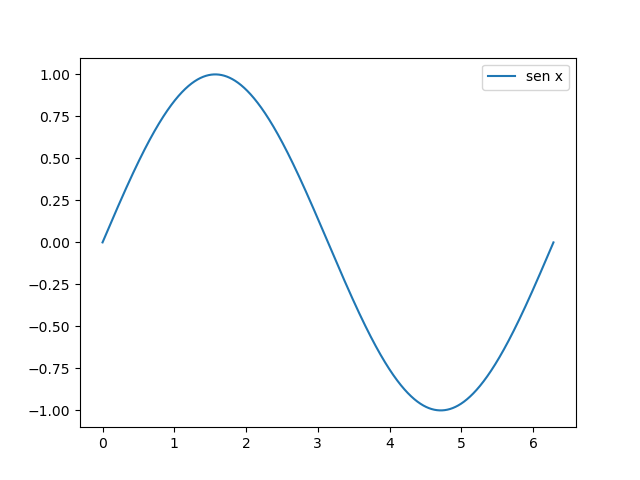
\includegraphics[scale=0.8]{figuras/Figure_1.png}
        \caption{Función trigonométrica seno de $0$ a $2\pi$}
        \label{fig:funcion_seno}
    \end{figure}
   \newpage
    \subsection{Tablas}
\href{https://www.tablesgenerator.com/}{Enlace para tablas en línea}


\begin{table}[h!]
    \caption{ Parámetros obtenidos después de pruebas de esfuerzo para dos muestras de microfilamentos esterilizados de tejidos musculares. Fuente: \cite{Rojas2022}  \\}
    \label{tabla:ejemplo_1} 
    \centering
        \begin{tabular}{c m{2cm} c c}
            \toprule
            Muestra                &  \centering Esfuerzo mecánico (\si{\mega\pascal})          & Límite elástico (\si{\mega\pascal})        & Tensión de rotura (\si{\mega\pascal})         \\ \midrule
            PCL 25 \si{\kilo\gray} & \num{1716(353)} & \num{236} $\pm$ \num{68} & \num{298(104)} \\
            PCL 0 \si{\kilo\gray}  & \num{2337 (397)}  & \num{284 (36)} & \num{325(39)}   \\ \bottomrule
    \end{tabular}
\end{table}
      

\subsection{Código computacional}

\begin{algorithm}[h!]
        \caption{Ejemplo del uso de \textit{docstrings}}
    \begin{minted}{python}
    def DistribucionUniforme(nNumeros = 10000):
    """
    Generar una distribución uniforme de números aleatorios. 
    Esto es un docstring.
    """
    # Generar números aleatorios con una semilla determinada
    np.random.seed(32423)
    \end{minted}
\end{algorithm}
\newpage

